% Resume imprimable du portfolio (2 pages A4). Compiler : xelatex resume_portfolio.tex (dans outils/resume/)
\documentclass[10pt,a4paper]{article}
\usepackage[margin=14mm,top=12mm,bottom=12mm]{geometry}
\usepackage{fontspec}
\setmainfont{Source Sans 3}[BoldFont={Source Sans 3 SemiBold}]
\newfontfamily\titre{Lora}[BoldFont={Lora SemiBold}]
\usepackage[french]{babel}
\usepackage{xcolor,graphicx,tikz,enumitem,tabularx,array}
\usepackage[hidelinks]{hyperref}\usepackage{needspace}
\definecolor{vert}{HTML}{1A6B3C}\definecolor{gris}{HTML}{5B655E}\definecolor{fond}{HTML}{E8F2EC}
\setlength{\parindent}{0pt}\setlength{\parskip}{3pt}
\setlist{nosep,leftmargin=12pt,itemsep=1.5pt}
\pagestyle{empty}
\newcommand{\rubrique}[1]{\needspace{7\baselineskip}\vspace{7pt}{\titre\large\bfseries\color{vert}#1}\par\vspace{-2pt}{\color{vert}\rule{\linewidth}{0.6pt}}\par\vspace{2pt}}
\newcommand{\projet}[3]{\vspace{4pt}{\bfseries #1}\hfill{\small\color{gris}#2}\par{\small\color{gris}#3}\par}
\newcommand{\cle}[1]{\colorbox{fond}{\parbox{\dimexpr\linewidth-2\fboxsep}{\small #1}}\par}
\begin{document}

% ---------------- en-tete ----------------
\begin{minipage}[c]{27mm}
\begin{tikzpicture}\clip (0,0) circle (12.5mm); \node at (0,0) {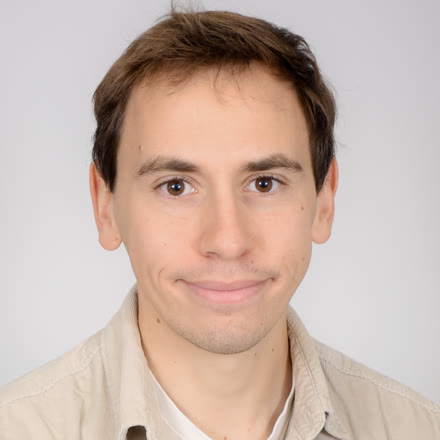
\includegraphics[width=25mm]{../../images/photo_jeremy.jpg}};\end{tikzpicture}
\end{minipage}\hspace{4mm}%
\begin{minipage}[c]{\dimexpr\linewidth-31mm}
{\titre\fontsize{24}{26}\selectfont\bfseries Jérémy Genty}\par\vspace{2pt}
{\large\color{gris}Données climatiques, environnement et forêt}\par\vspace{4pt}
\small\href{mailto:genty.jeremy36@gmail.com}{\color{vert}genty.jeremy36@gmail.com}\quad·\quad
\href{https://www.linkedin.com/in/j%C3%A9r%C3%A9my-genty/}{\color{vert}LinkedIn}\quad·\quad
\href{https://github.com/jeremygenty36-boop}{\color{vert}github.com/jeremygenty36-boop}\quad·\quad Permis B
\end{minipage}

\vspace{6pt}
Diplômé du Master Agrosciences, Environnement, Territoires, Paysage, Forêt (Université d'Orléans, 2026), je travaille à la croisée du climat, de la forêt et des données. Pendant mon stage à l'UMR Silva, j'ai étudié l'effet de la chaleur, du froid et de la sécheresse sur la mortalité des arbres ; auparavant, j'ai passé six mois sur le terrain en santé des végétaux. Curieux, proactif et créatif, j'aime proposer et construire des outils, avec un esprit critique sur les données et le goût de la pédagogie.

\rubrique{Ce que je sais faire}
\begin{tabularx}{\linewidth}{@{}>{\bfseries}p{36mm}X@{}}
Analyser des données & Grands jeux de données climatiques et forestiers sous R (terra, NetCDF), modèles statistiques (GLM, sélection, validation croisée). \\
Cartographier & QGIS, PostGIS, SQL ; télédétection Sentinel-2 (NDVI, Orfeo ToolBox) ; cartes web interactives. \\
Aller sur le terrain & Relevés de flore et phytosociologie, piégeage et identification d'insectes, contrôles phytosanitaires. \\
Transmettre & Rapports, notes de synthèse, posters, présentations orales, supports pédagogiques. \\
\end{tabularx}

\rubrique{Projets principaux}
\projet{Extrêmes climatiques et mortalité des arbres}{Stage de M2 · UMR Silva, Nancy · 2026}{6 indices d'extrêmes calculés avec 5 bases climatiques (dont 2 descendues à 1 km), mortalité de 8 essences modélisée sur 21\,989 placettes de l'Inventaire forestier national.}
\begin{itemize}
\item \textbf{Même performance, lecture différente} : les 5 bases expliquent la mortalité aussi bien (AUC 0,758 à 0,763), mais pour 6 essences sur 8 l'extrême dominant change selon la base.
\item Les bases s'accordent sur l'intensité (R² 0,85 à 0,87), beaucoup moins sur la fréquence des vagues et la sécheresse (R² 0,14 à 0,6).
\item Le climat reste secondaire (8,2 \% de l'explication, la structure du peuplement domine) ; les extrêmes ne font pas mieux que le climat moyen.
\item Chaîne de traitement publiée en accès libre, avec un registre de 17 erreurs corrigées (ERRATA).
\end{itemize}

\projet{Carte interactive des extrêmes climatiques en France, 1979-2024}{Projet personnel · 2026}{6 indices recalculés depuis E-OBS (11 Go de données journalières) ; carte web avec tendances, extrêmes décennaux, lien avec les modèles de mortalité du stage et mortalité observée par département.}
\cle{Les journées les plus chaudes de l'année ont gagné 0,8~°C par décennie en France depuis 1979 ; les vagues de chaleur sont passées de 1,4 à 5 par an.}

\projet{Technicien spécialisé : inspections phytosanitaires}{FREDON Centre-Val de Loire · juin-déc. 2022}{Contrôles du passeport phytosanitaire européen chez des horticulteurs, pépiniéristes et jardineries ; relevés JEVI ; comptes rendus d'inspection, par délégation de la DRAAF.}

\projet{Cartographie des incendies de 2022 dans les Landes}{M1 · avec Pierre Sergent · 2023-2024}{Sentinel-2, différence de NDVI, masque forêt OSO, QGIS et Orfeo ToolBox, validation par photo-interprétation : 3\,538~ha brûlés mesurés à La Teste-de-Buch (3\,500~ha selon la presse), précision de 93,8~\% en surface.}

\projet{Phytosociologie des prairies et pelouses du Loiret}{M1 · avec Claire Bellin · 2023-2024}{258 relevés, classification hiérarchique, 11 groupements végétaux rattachés à des syntaxons, écogrammes et conseils de gestion.}

\projet{Un fongicide biologique nuit-il aux insectes auxiliaires du verger ?}{Stage de M1 · Gembloux Agro-Bio Tech (Erasmus+) · 2024}{1\,813 insectes de 31 familles sous quatre traitements : pas de différence de communauté (p = 0,276), la météo pèse plus que le traitement.}

\rubrique{Autres travaux de formation}
\begin{itemize}
\item Phylogéographie du capricorne asiatique (\textit{Anoplophora}) : PCR, séquençage COI, arbres phylogénétiques (poster M1).
\item Restauration écologique de la carrière de Sandillon : inventaires oiseaux, carabes, reptiles, flore ; analyses sous R (M1).
\item Cartographie des habitats de la carrière de Courpain : relevés GPS, carte QGIS (L3).
\item Rouille du peuplier (pathotypage) et 25 fiches de diagnostic des maladies des végétaux (M1).
\item Résistance à la sécheresse du peuplier (P50, courbes de vulnérabilité sous R) selon la fertilisation azotée (M1).
\end{itemize}

\rubrique{Formation}
\projet{Master Agrosciences, Environnement, Territoires, Paysage, Forêt}{Université d'Orléans · 2023-2026}{Stage de M2 noté 16,3/20. 1\textsuperscript{er} de promotion en Biologie évolutive et génétique des populations (16,5), Réseaux écologiques (15,75) et Génomique des écosystèmes forestiers (15,5) ; 2\textsuperscript{e} en Écologie des communautés (17,5).}
\projet{Licence Sciences de la vie : biologie des organismes, populations et écosystèmes}{Université d'Orléans · 2019-2023}{}

\rubrique{Langues, outils et centres d'intérêt}
\textbf{Langues} : français (maternelle), anglais B2/C1, allemand A2.\quad
\textbf{Outils} : R, QGIS, PostGIS, SQL, Python (en apprentissage), Zotero, LaTeX.\par
\textbf{Centres d'intérêt} : botanique, ornithologie, vélo, course à pied, randonnée.\par
\rubrique{En images}
\begin{minipage}[t]{0.31\linewidth}\centering
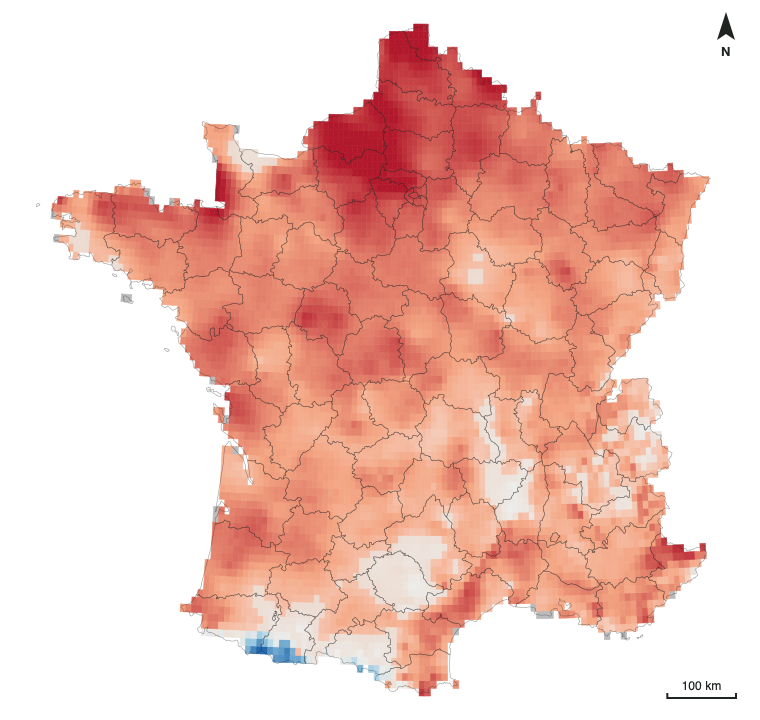
\includegraphics[width=\linewidth]{../../images/carte_txx_tendance.png}\par\vspace{2pt}
{\footnotesize\color{gris}Tendance des extrêmes de chaleur (TXx) en France, 1979-2024 : rouge = réchauffement (carte interactive, données E-OBS).}
\end{minipage}\hfill
\begin{minipage}[t]{0.31\linewidth}\centering
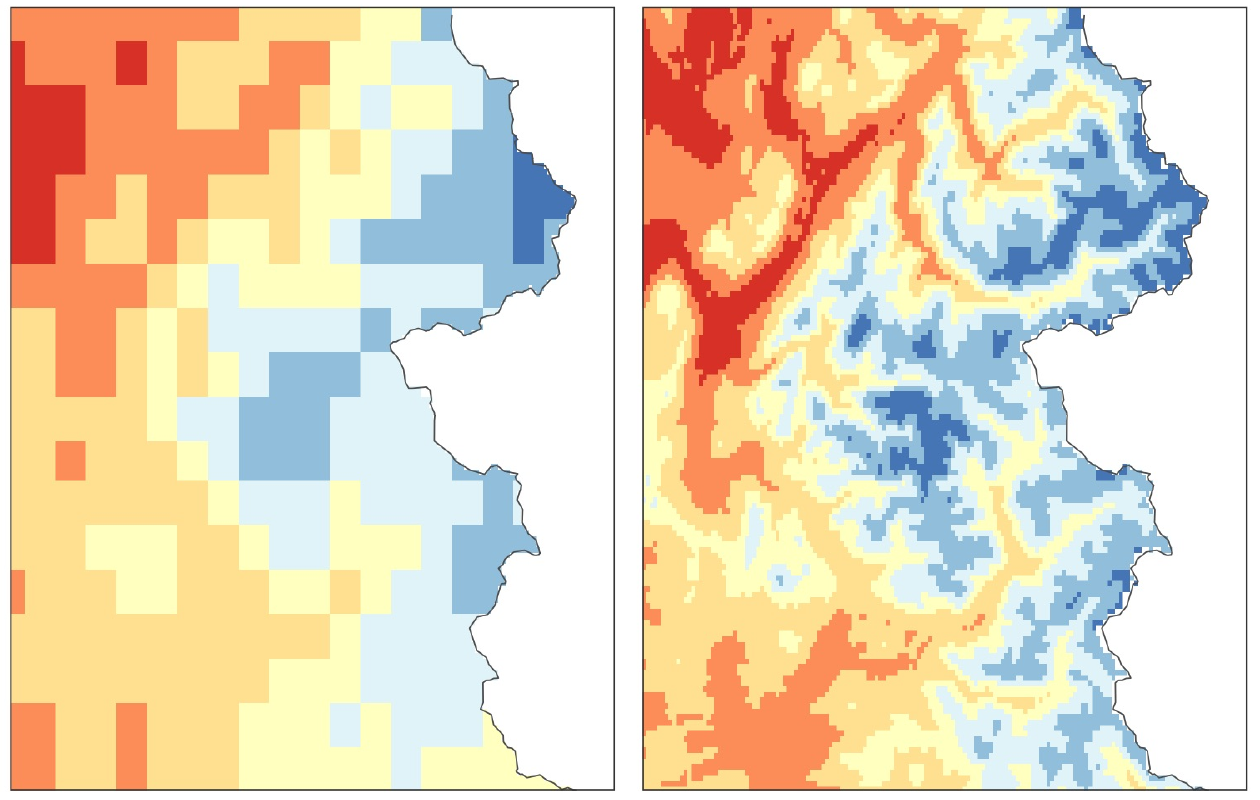
\includegraphics[width=\linewidth]{../../images/descente_echelle_alpes.png}\par\vspace{2pt}
{\footnotesize\color{gris}Descente d'échelle de 8 km à 1 km (Tmin 2014, Alpes du Nord) : les vallées et les crêtes apparaissent (stage de M2).}
\end{minipage}\hfill
\begin{minipage}[t]{0.31\linewidth}\centering
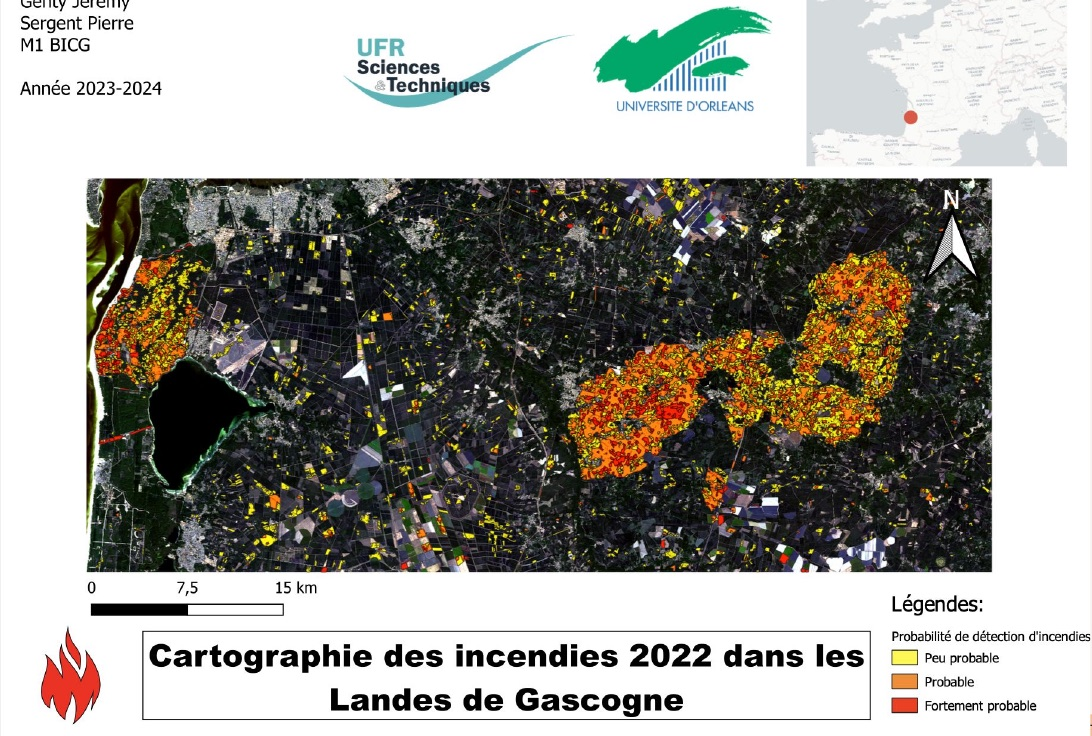
\includegraphics[width=\linewidth]{../../images/landes_incendies_2022.jpg}\par\vspace{2pt}
{\footnotesize\color{gris}Surfaces brûlées en 2022 dans les Landes de Gascogne, détectées sur images Sentinel-2 (projet de M1).}
\end{minipage}

\vspace{6pt}
\begin{minipage}[t]{0.48\linewidth}\centering
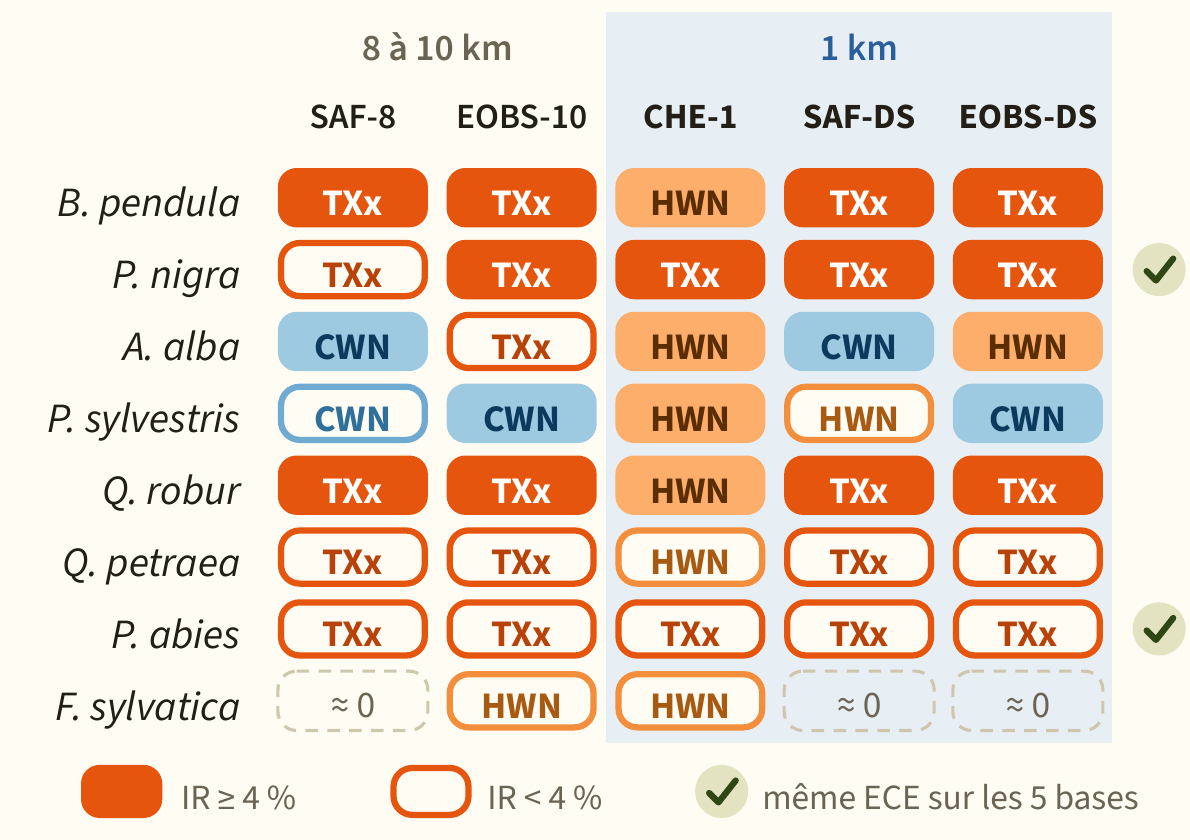
\includegraphics[width=\linewidth]{../../images/ece_dominant_par_base.png}\par\vspace{2pt}
{\footnotesize\color{gris}L'extrême le plus important du modèle de mortalité change selon la base climatique pour 6 essences sur 8 (poster de M2).}
\end{minipage}\hfill
\begin{minipage}[t]{0.48\linewidth}\centering
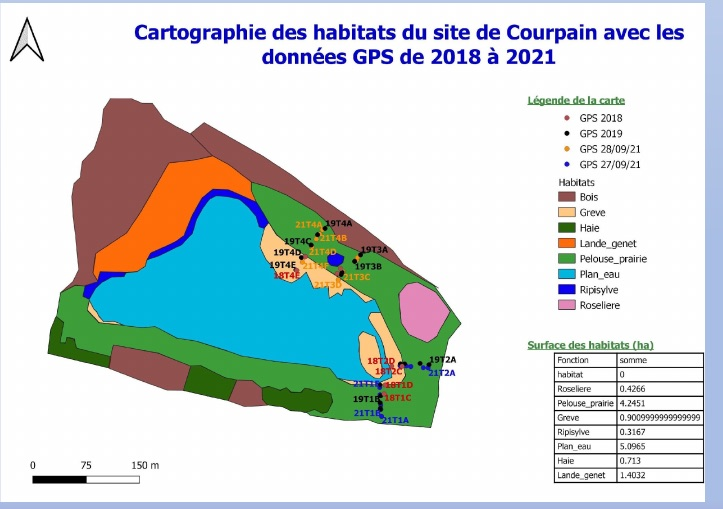
\includegraphics[width=\linewidth]{../../images/courpain_habitats.jpg}\par\vspace{2pt}
{\footnotesize\color{gris}Carte des habitats d'une ancienne carrière (Courpain), d'après des relevés GPS et sous QGIS (L3).}
\end{minipage}

\vspace{4pt}{\small\color{gris}Références disponibles sur demande : encadrants de mes stages de Master 2 et de Master 1. Portfolio en ligne avec la carte interactive, les rapports et les posters.}

\end{document}
